%------------------------------------------------------------------------------
% Author(s):
% Varaun Ramgoolie
%
% Copyright:
%  Copyright (C) 2020 Brad Bachu, Arjun Mohammed, Varaun Ramgoolie, Nicholas Sammy
%
%  This file is part of Applied-Mathematics-Unit2 and is distributed under the
%  terms of the MIT License. See the LICENSE file for details.
%
%  Description:
%     Year: 2005 C
%     Module: 3
%     Question: 6 Sketch 1
%------------------------------------------------------------------------------

\documentclass[crop,tikz]{standalone}
\usetikzlibrary{scopes,calc,patterns,angles,quotes}

\begin{document}
	

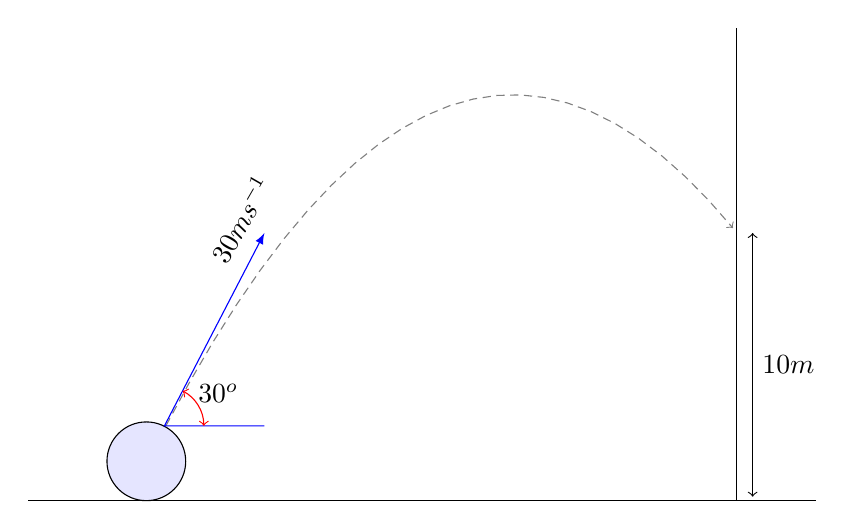
\begin{tikzpicture}
	\draw (-5,0) -- (5,0);
	\draw (4,0) -- (4,6);
	
	
	
	% ball
	\draw [draw=black,fill=blue!10] (-3.5,0.5) circle [radius=0.5];
	
	
	
	% ball path and reference
	\draw  [->, domain=-3.25:3.95, densely dashed,gray,font=\small] plot (\x, {-(13/60)*(\x-2)*(\x-2)+(-11/30)*(\x-2) + 5});
	
	\draw [<-, >=latex,draw=blue] (-2, 3.4) coordinate(x_1) -- (-3.27, 0.95) coordinate(x_2) -- (-2,0.95) coordinate (x_3);
	
	\node[rotate=60, yshift=10] at (x_1)  {$30 ms^{-1}$};
	
	
	
	% drawing angle
	\path 
	(x_1)
	-- (x_2)
	-- (x_3)
	pic["$30^o$",draw=red,<->,angle eccentricity=1.6,angle radius=0.
	5cm] {angle=x_3--x_2--x_1};



	% arrow showing 10m	
	\coordinate (a) at (4.2,-0.25);
	\coordinate (b) at (4.2,3.1);
	\draw[<->] ([yshift=0.3cm]a) -- ([yshift=0.3cm]b) node[midway,right]{$10m$};
	 
\end{tikzpicture}	
	
	
	
	
\end{document}

